\begin{figure*}[t]
  \centerline{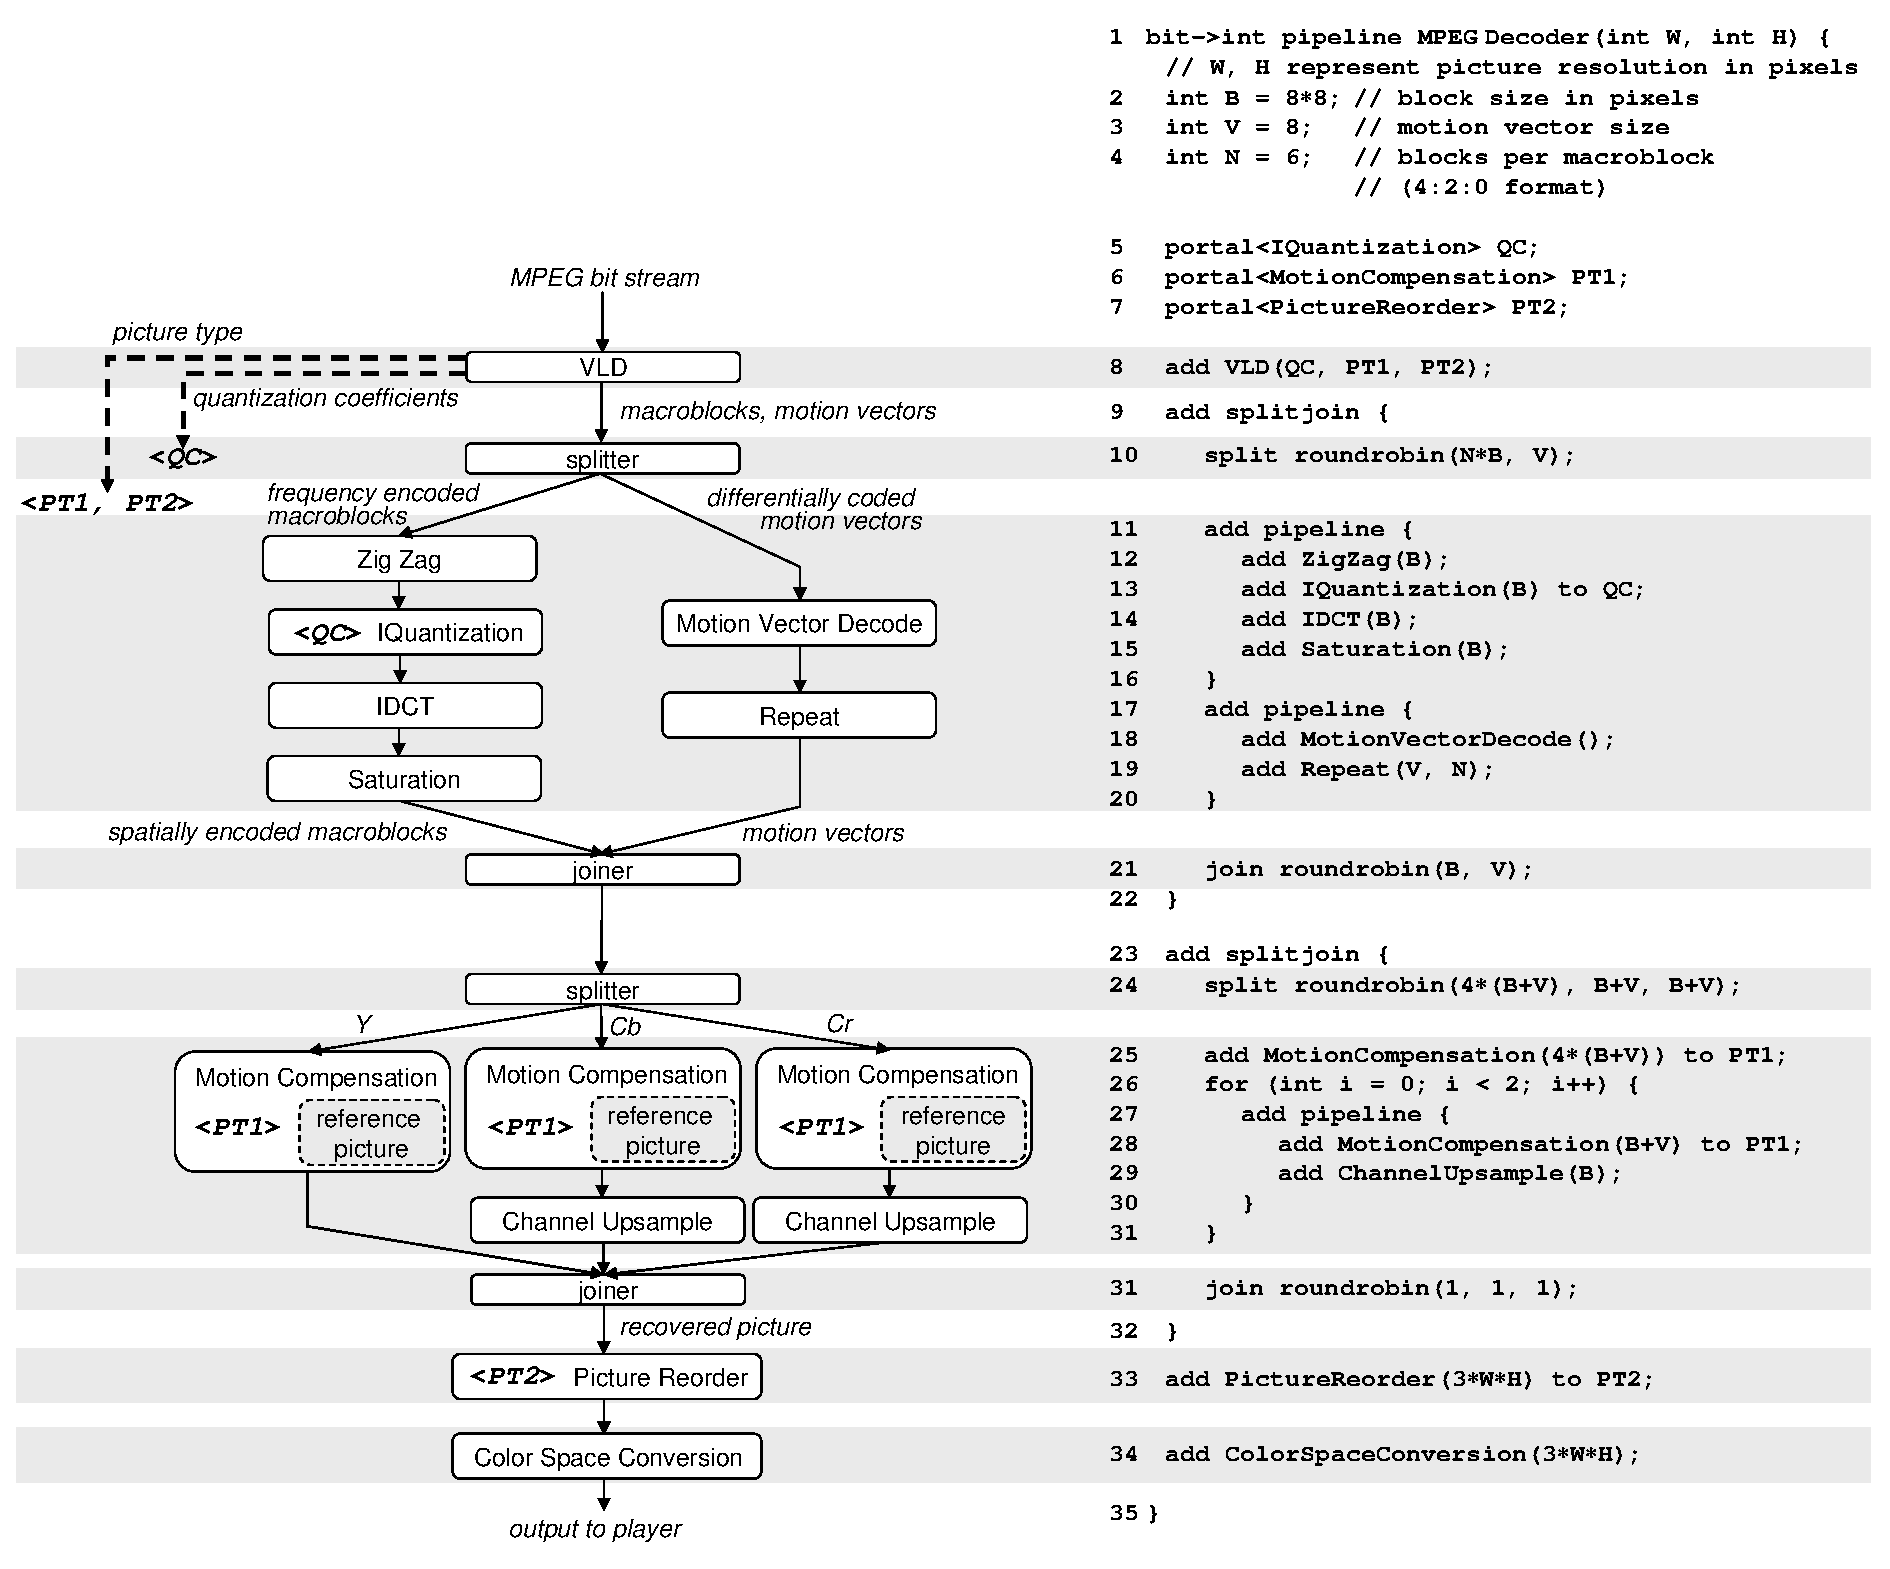
\epsfig{file=decoder_with_code.eps,width=\textwidth}}
  \caption{MPEG-2 decoder block diagram and corresponding StreamIt code.}
  \label{fig:dec-with-code}
\end{figure*}

\Section{MPEG Decoder in StreamIt}

The MPEG decoder pipeline is shown in
Figure~\ref{fig:dec-with-code}. The stream graph is shown on the
left. The StreamIt code is shown on the right, and it is correlated
with the stream block level diagram.

%% The decoder accepts a compressed bit stream as input, and produces the
%% decoded video stream as output.
The computation is encapsulated in three main components:
the parser (line 8), the block and motion vector decoder (lines 9-22),
and the motion compensator (lines 23-32).
The parser is responsible for parsing the MPEG-2 bit stream and
performing Huffman and variable run-length decoding (VLD). The output
of the VLD is an interleaved stream of quantized macroblocks encoded
in the frequency-domain, and offset-encoded motion vectors. The VLD
outputs $\texttt{N}\times\texttt{B}$ data elements for each
macroblock, followed by \texttt{V} data elements that encode its
motion vector. The actual value of \texttt{N} depends on the chroma
format. In a 4:2:0 chroma format regime, $\texttt{N}=6$ since each
macroblock consists of four 8x8 subpixel blocks for the luminance
channel, and two 8x8 subpixel blocks for the two chrominance
channels. Therefore, the VLD outputs a total of six 8x8 blocks, or 384
subpixels per macroblock. However, the total number of macroblocks
that are output by the parser is dependent on the number of frames in
the input encoded video. As a result, the VLD has a variable I/O
rate. The VLD filter is the only variable rate filter in the decoder
pipeline.

The VLD output is segregated into two homogeneous streams by a
roundrobin splitter (line 10). The first stream undergoes inverse
transformations (lines 11-16), while the second is decoded to produce
absolute motion vectors (lines 17-20). As is evident from the computation
graph, the two streams are decoded in parallel, and then merged (line
21) prior to the motion compensation stage of the pipeline.

The inverse transformations map each 8x8 block from the frequency
domain back to the spatially encoded domain. Each block is reordered
(line 12), and then inversely quantized (line 13). This is followed by
an inverse DCT and a bounded saturation filter (lines 14-15). The set
of transformations is grouped into a pipeline whose input
and output types are automatically inferred by the compiler. Each of
the filters in this pipeline operate on 8x8 blocks. The code that is
shown does not take advantage of data level parallelism between
blocks. It is rather straightforward however to expose this
parallelism if it is desirable. For example, in this case a splitjoin
can replicate the inverse transformation pipeline $N$ times:
\begin{center}
  \begin{scriptsize}
    \begin{verbatim}
      add splitjoin {
        split roundrobin(B);
        for (int i = 0; i < N; i++) 
        // add pipeline
        join roundrobin(B);
      }
    \end{verbatim}
  \end{scriptsize}
\end{center}
A stream-aware compiler can also automatically adjust the execution
granularity as necessary~\cite{gordon02asplos}, since data-parallel streams
can be easily identified as those that are stateless (i.e., do not
carry mutable state from one iteration to the next).

The third stage of the decoding pipeline performs the motion
compensation (lines 23-32) to recover predictively coded
macroblocks. The motion compensation filter uses the motion vectors to
find a corresponding macroblock in a previously decoded reference
picture. The reference macroblock is added to the current macroblock
to recover the original picture data. If the current macroblock is
part of an I or P picture, then the decoder stores it for use as a
future reference picture.

In the compensation stage, there are three parallel streams.  The
first handles the luminance color channel (Y), and the other two
handle the chrominance channels (Cb and Cr). The roundrobin splitter
(line 24) distributes the macroblocks according to the chroma
format. Since the luminance channel is not downsampled during the
encoding process, the splitter dispatches four 8x8 blocks at a time to
the Y motion compensator. The chrominance channels are typically
downsampled by a factor of 4, and hence one 8x8 block is streamed to
each of the Cb and Cr pipelines, which upsample (line 29) the results
of the motion compensator to generate the full 16x16 macroblock.  The
upsampling is a linear interpolation of the surrounding pixels.
The joiner (line 31) assembles the pictures from each of the color
channels, one pixel at a time.  The output is then readied for display
(lines 33 and 34) by organizing the pictures in accord with their
temporal order, and performing color space conversion to the RGB (red,
green, blue) color model. Note that these two filters each consume
$3\times\texttt{W}\times\texttt{H}$ subpixels per picture. This is
three times the pixel resolution of the decoded image since there is
one pixel generated from each of the three channel decoders. The final
output of the decoder is $\texttt{W}\times\texttt{H}$ pixels.  In
contrast to the filters for motion compensation and inverse transformation,
whose I/O rates are statically resolved at compile time, the picture 
reordering and color space conversion have I/O rates that are
parameterized on initialization time constants; namely the pixel
resolution of the pictures.

%% The MPEG-2 decoder in StreamIt is a fully portable implementation in
%% that the application is not architecture dependent. The implementation
%% naturally exposes the pipeline parallelism that exists throughout the
%% decoder, as well as the data level parallelism inherent to the inverse
%% transformations and motion compensation.  

The decoder implementation was carried out by one student programmer
with no prior understanding of MPEG. The development spanned eight
weeks from specification~\cite{MPEG2} to the first fully functional
MPEG decoder. The StreamIt code is nearly 3,165 lines of code with 48
static streams. The bit stream parser is the largest single filter,
consisting of 775 lines of code. The 48 static streams compile to
2,150 instantiated filters\footnote{A  {\it static stream} is a unique
code block, which may have multiple  instantiations when compiled. For
instance the \texttt{MotionCompensation()}  filter is one static
stream, but is instantiated three times.} at a picture resolution of
352x240. By way of comparison, the reference C
implementation~\cite{reference-mpeg-c} is 6,835 lines of
code\footnote{Line counts were generated using  the \texttt{SLOCcount}
tool. It strips whitespace and comments.}.  A line count comparison is
not an accurate measure of programmability, since our StreamIt decoder
implements only a subset of several stream types supported by MPEG.
Our decoder does provide full support for the range of different
compression techniques used within MPEG, but supports only a subset of
the possible display modes (i.e. interlaced versus progressive
output).  However, these alternate display formats represent minor
conceptual changes and should therefore affect small portions of the
StreamIt code. This is demonstrated in Section~\ref{section:chroma}
with an example that illustrates how to support multiple chrominance
formats.

The reference C implementation intermingles parsing, decoding, and
motion compensation, making it difficult to clearly follow the code,
and hindering a better comparison. The C code also relies on global
variables to communicate values, such as quantization coefficients,
from the parser to the relevant code regions. In StreamIt, such
communication is relegated to teleport messaging (lines 13, 25, 28, and
33, and illustrated with dotted lines in
Figure~\ref{fig:dec-with-code}). For instance, the parser (VLD)
generates a message whenever the picture or macroblock type
changes. The motion compensation filters receive this information via
their dedicated portal (line 28), determine how to process the current
picture, and decide whether they needs to store the picture for future
reference. Note however that while there are multiple motion compensators
subscribed to the same portal, they each receive the same message with
respect to their local execution.
The picture reordering filter receives a similar message
(via portal on line 33), and uses the information to determine the
correct temporal order of pictures. The inverse transformation
pipeline listens to its portal (line 13) to determine the algebraic
manipulation required to perform the inverse quantization of the input
macroblock. Teleport messaging 
%% proves as a natural mechanism because
%% the macroblock type and picture type information changes infrequently
%% and irregularly, compared to the regular flow of data in the
%% application. Moreover, by 
exposes the flow of messages to the compiler, and allows for large
scale reordering or parallelization of the application without a
heroic dependence analysis. It also provides a mechanism to easily
dynamic behavior into an otherwise static processing pipeline.

In StreamIt, all of the processing is encapsulated hierarchically into
single-input, single-output streams with well-defined modular
interfaces. This property facilitates development and boosts
programmer productivity, as components can be debugged and verified as
standalone components. The modularity also promotes reuse. For
example, the zig-zag descrambler and inverse DCT
components may be used as is to implement a JPEG decoder.

%% \SubSection{Motion Compensation}

% Commented out this section since this information is incorporated into
% the decoder implementation section. - Matt 1/25/06
% An MPEG decoder accepts a bitstream as input and performs Huffman and
% variable run-length decoding (VLD).  This process results in a set of
% quantized, frequency-domain macroblocks and corresponding motion
% vectors.  The decoder inversely quantizes (IQ) the macroblocks and then
% performs an inverse DCT (IDCT) to convert the macroblocks to the
% spatial domain.  For predictively coded macroblocks (e.g., P and B
% pictures), the decoder performs motion compensation (MC) using the
% input motion vectors to find a corresponding macroblock in a
% previously decoded, stored reference picture. This reference
% macroblock is added to the current macroblock to recover the original
% picture data. If the current macroblock is part of an I or P picture,
% then the decoder stores it for future reference.
% Figure~\ref{fig:dec_block} illustrates the decode sequence.

%\begin{figure}[htbp]
%\centerline{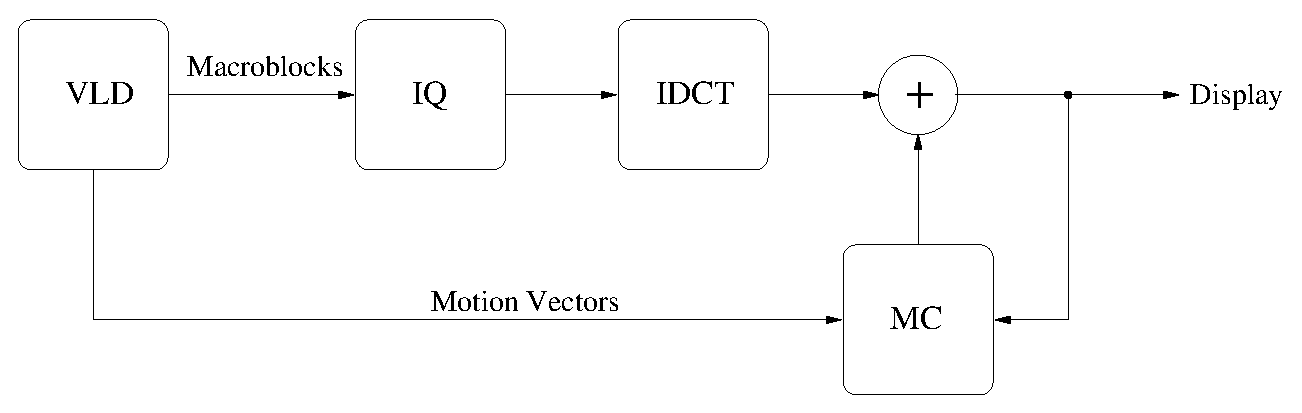
\epsfig{file=dec_block.eps,width=5in}}
%\caption{Block diagram of MPEG-2 decode.}
%\label{fig:dec_block}
%\end{figure}

%% A simple strategy for parallelizing the MPEG-2 decoding can exploit
%% the data parallelism among macroblocks. Using this scheme, the Huffman
%% and run-length decoding is inherently serial, as macroblock boundaries
%% can only be discovered by performing the decode operation.  Once this
%% decode is complete, a parallel implementation can distribute
%% macroblocks to independent streams (using a splitjoin). Each stream
%% performs the inverse quantization, inverse discrete cosine transform,
%% and motion compensation. Furthermore, each stream locally stores
%% reference macroblocks for future motion compensation. Using this
%% strategy, the streams can execute independently with one exception.

%% % TODO: This is the figure showing the macroblock parallelism
%% % I'm not sure where it goes. - Matt
%% \begin{figure*}[t]
%% \vspace{-12pt}
%% %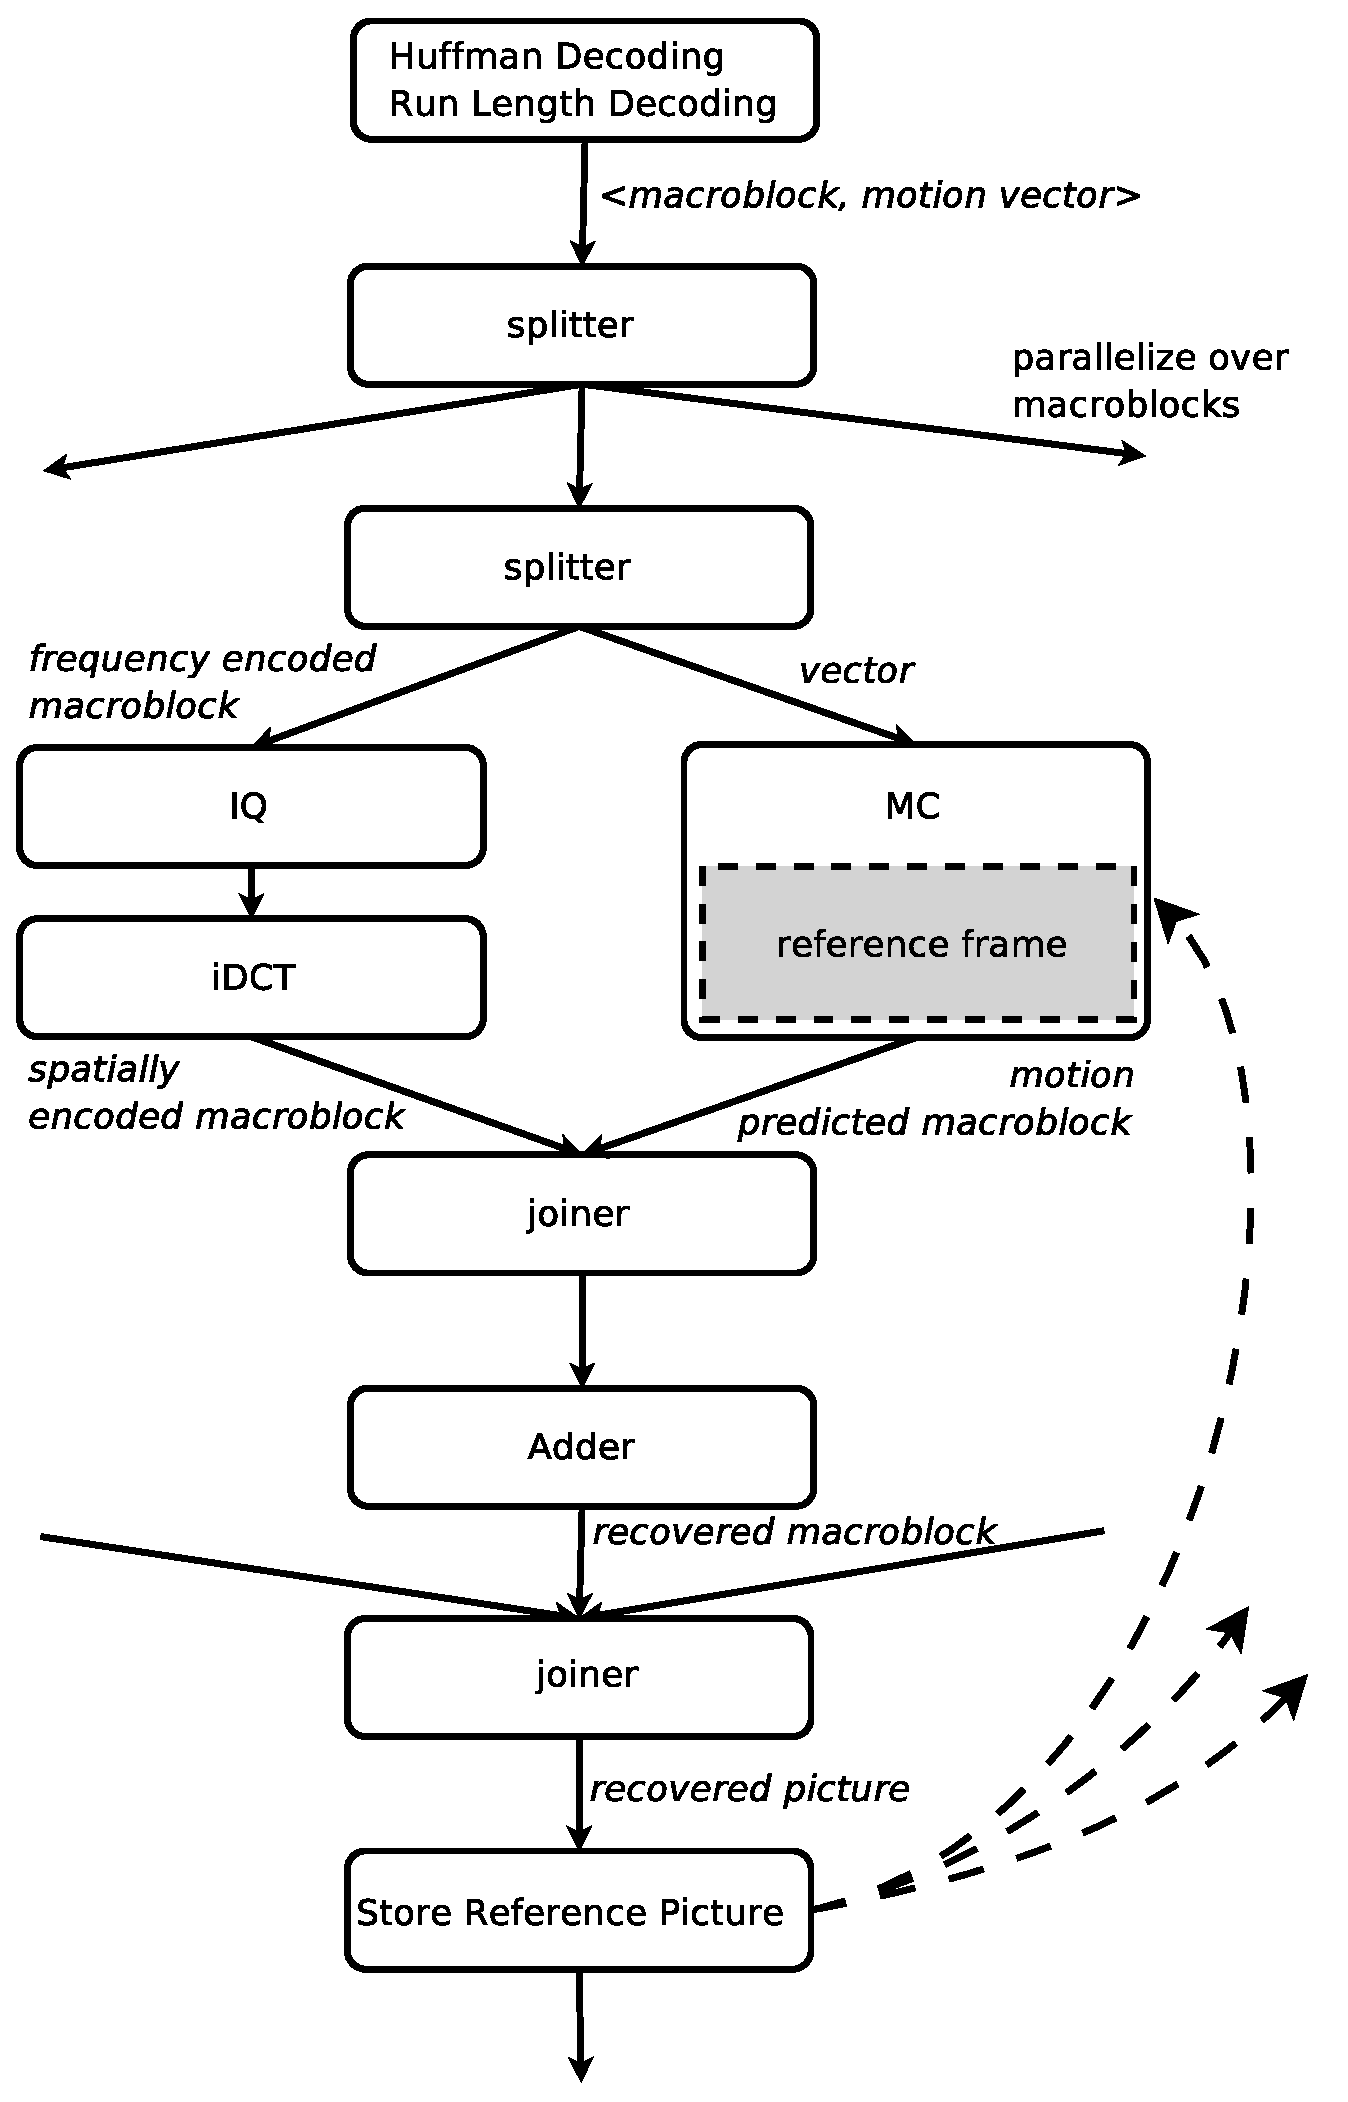
\epsfig{file=decoder_macroblock_parallelism.eps, width=3in}
%% %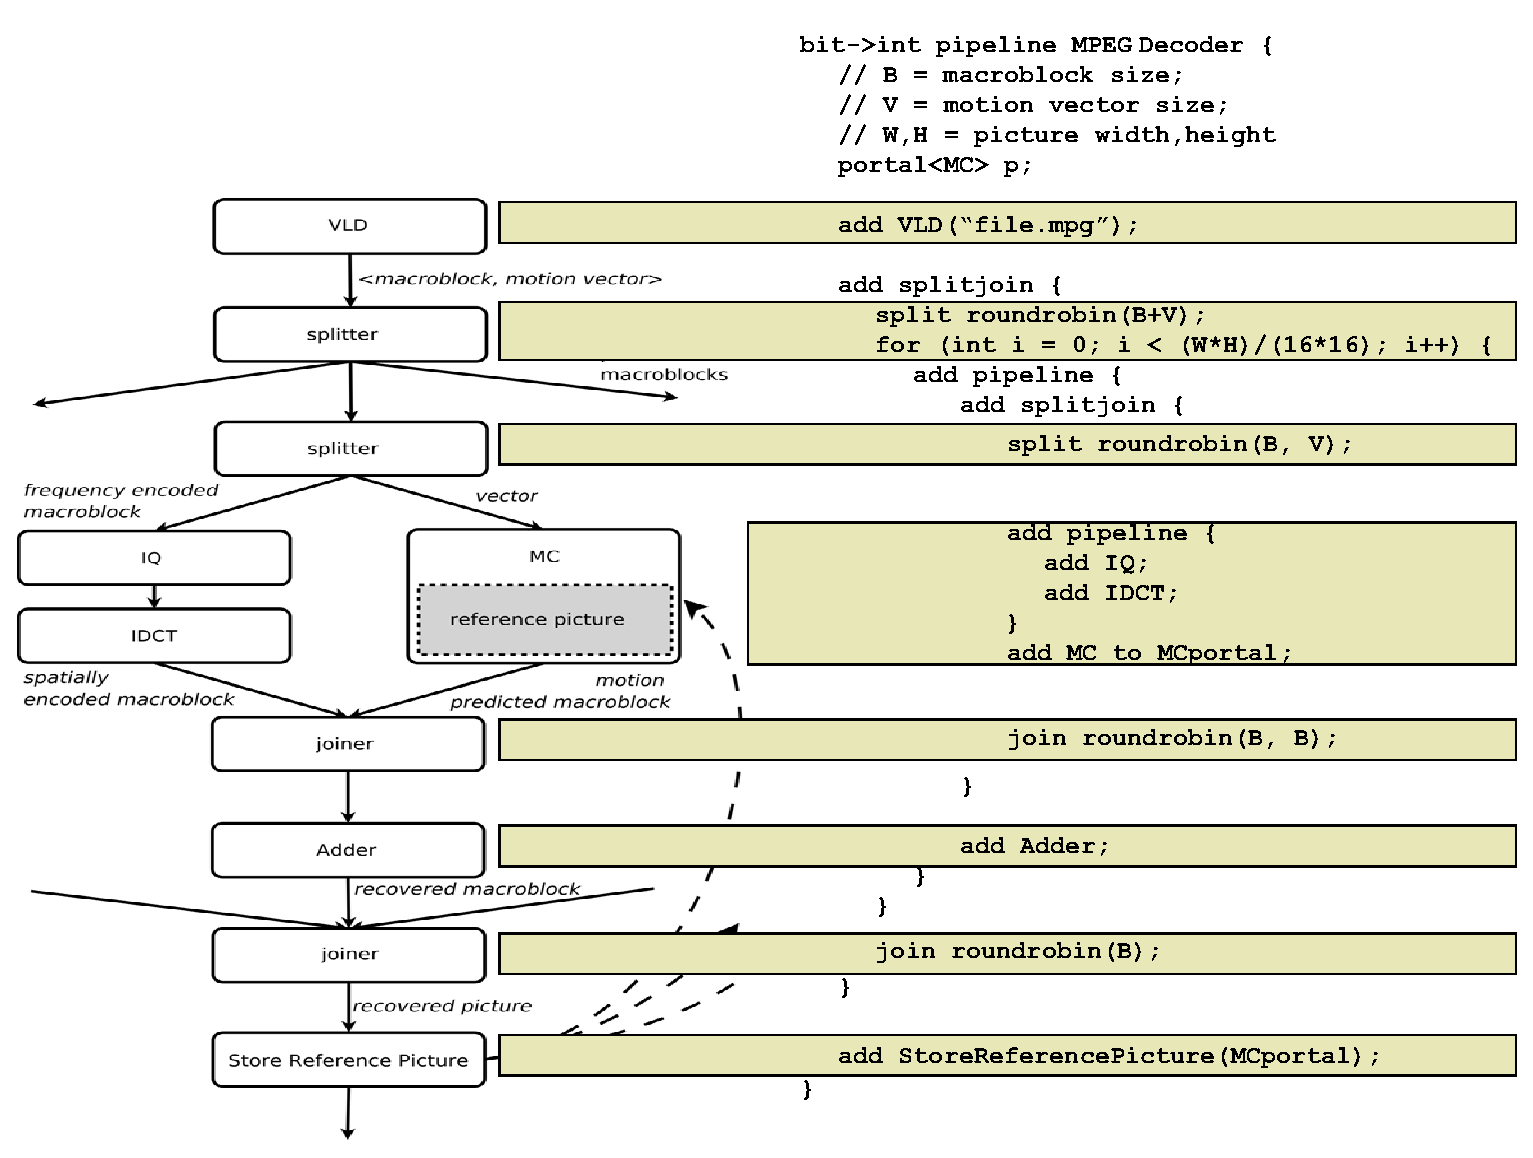
\epsfig{file=decoder-parallel.eps, width=\textwidth}
%% 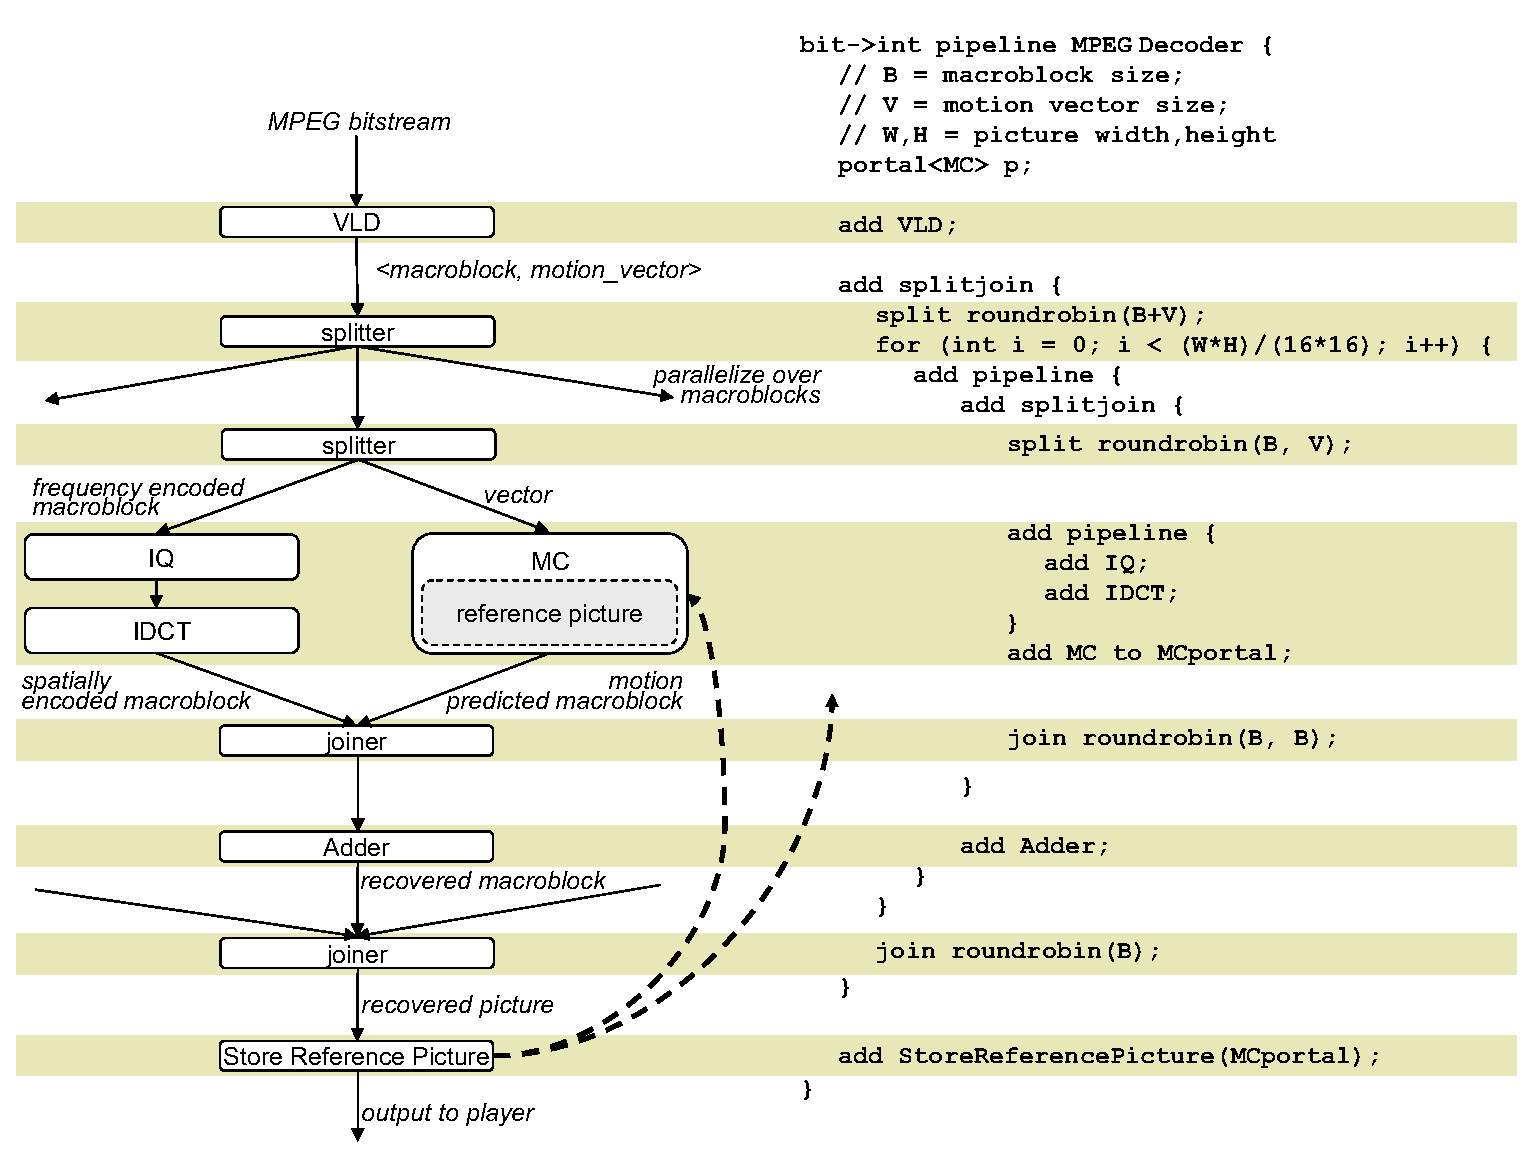
\epsfig{file=decoderpipeline.eps, width=\textwidth}
%% % TODO: Change Matt's 2 am caption.
%% \caption{MPEG-2 decoder exploiting macroblock-level parallelism.}
%% \label{decoder_macroblock_parallelism}
%% \vspace{-6pt}
%% \end{figure*}

%% This exception occurs when a stream is performing motion compensation
%% and the corresponding motion vector indicates a reference macroblock
%% stored in some other stream. In this case, inter-stream communication
%% is required to send the reference data to the requesting stream. This
%% situation is not uncommon, and is more prevalent for higher resolution
%% pictures. A simple scheme for handling this situation is for every
%% stream to broadcast its decoded macroblocks to all other streams. This
%% solution has the benefit of being conceptually easy to understand and
%% implement. StreamIt allows programmers to naturally expose such
%% parallelism.
%% A StreamIt pipeline that operates at macroblock
%% granularity is shown in Figure~\ref{decoder_macroblock_parallelism}. It is
%% worthy to note that there is a high correlation between the stream
%% graph, and the StreamIt syntax describing the pipeline.

%% The implementation can be made more fine grained by exposing the
%% intra-macroblock parallelism. For example, the IQuantization-IDCT
%% pipeline can operate at a block level, rather than at a macroblock
%% granularity. This is easily achieved by encapsulating the  pipeline
%% within a splitjoin to scatter the blocks, operate, and gather the
%% results to recover the parent macroblock.

%% There are many implementation strategies for the decoder, each with
%% varying degrees of exposed parallelism. Of the greatest advantage of
%% the StreamIt implementation is its malleability. The stream graph is
%% easily reconfigured to operate at picture-level granularity (exposing
%% parallelism between chroma channels), macroblock level (exposing even
%% more data-level parallelism), or even at block level (exposing the
%% greatest amount of data-level parallelism).